\documentclass[12pt, a4paper, onecolumn, oneside, toc=bibliographynumbered, liststotoc]{scrreprt} %Schriftgröße 12pt, DIN A4, 1 Spalte, einseitig bedruckt, Literaturverzeichnis in Inhaltsverzeichnis eintragen mit Nummerierung als Anhang

\usepackage[T1]{fontenc} %Codierung für deutsche Schriftzeichen
\usepackage[utf8]{inputenc} % UTF-8 Encoding
\usepackage[ngerman]{babel} % Neue Deutsche Rechtschreibung
\usepackage[onehalfspacing]{setspace} %1,5 Zeilen Zeilenabstand
\usepackage{scrlayer-scrpage} %Kontrolle von Fuß- und Kopfzeile
\usepackage{graphicx} %Einfügen von Bildern
\usepackage{float} %Positionierung von Bildern
\usepackage[printonlyused, nohyperlinks, smaller]{acronym} %Unterstützung für Abkürzungen und Abkürzungsverzeichnis - es werden nur verwendete Abk. gedruckt
\pagestyle{scrheadings} %Seitenstil
\chead*{\pagemark} %Kopfzeile Mitte - Seitenzahl
\cfoot*{} %Fußzeile Mitte - leer
\usepackage{geometry}
\geometry{
  left=4cm,
  right=2cm,
  top=2cm,
  bottom=2cm,
%  bindingoffset=5mm
}
\usepackage[german=quotes]{csquotes}
\usepackage[backend=bibtex, citestyle=authoryear, bibstyle=authoryear, sorting=nty]{biblatex} %Angaben für Zitate - Nutzt Bibtex, Markierung auf Seite als alphanumerische Abkürzung, Sortierung nach Auftreten
\setcounter{biburllcpenalty}{9000}
\setcounter{biburlucpenalty}{9000}
\counterwithout{figure}{chapter}
\counterwithout{table}{chapter}
\addbibresource{Aufgabe_1.bib} %Bibliotheksdatei
%\addbibresource{WissArb.bib} %Bibliotheksdatei
% !!! Um Bibtex richtig zu verwenden, nach jeder Änderung in der .bib-Datei Bibtex laufen lassen !!!

%\setcounter{tocdepth} {4} % Inhaltsverzeichnis bis subsubsection
%\setcounter{secnumdepth}{4} % Nummerierung des Inhaltsverzeichnis bis subsubsection

\begin{document}
%Titelblatt und Inhaltsverzeichnis
\pagenumbering{roman} %Seitennummerierung i, ii, iii etc. 
	%Angaben für Maketitle
	\titlehead{Hochschule Rhein-Waal \\ %Hochschulinformationen
	Fakultät: Kommunikation und Umwelt\\
	Studiengang: Verwaltungsinformatik\\
	Modul: Workshop 2: Wissenschaftliches Schreiben\\}
%	\subject{Wissenschaftliches Arbeiten} %Art der Arbeit
	\title{Aufgabe 4\\
	Hausarbeit} %Titel
%	\subtitle{Einfallstore für Black Hat Hacker in Netzwerke} %Untertitel
	\author{Linus Wolf - 28611}
	\date{\today} %Datum (heute)
%	\publishers{Betreut durch Professor Frank Zimmer} %Betreuender Professor und zusätzliche Infos

\maketitle %Erzeuge Titelblatt (Ignoriert in scrreprt voreingestellte Kopf- und Fußzeile)
\newpage

%\newpage %Ende Abstract
\tableofcontents %Erzeuge Inhaltsverzeichnis (Bei Fehler erneut kompilieren - ToC braucht 2 Durchläufe)
\newpage

\listoffigures %Abbildungsverzeichnis
\newpage %Abschluss Titel und ToC - Neue Seite für Inhalt

	\addchap{Abkürzungsverzeichnis}
\begin{acronym}[RZF NRW]
\acro{bsi}[BSI]{Bundesamt für Sicherheit in der Informationstechnik}
\acro{fkie}[FKIE]{Fraunhofer-Institut für Kommunikation, Inforamtionsverarbeitung und Ergonomie}
\acro{ieee}[IEEE]{Institute of Electrical and Electronics Engineers.}
\acro{iot}[IoT]{Internet of Things}
\acro{lan}[LAN]{Local Area Network}
\acro{mac}[MAC]{Medium Access Control}
\acro{mbss}[MBSS]{Mesh Basic Service Set}
\acro{pan}[PAN]{Personal Area Network}
\acro{rfid}[RFID]{Radio Frequency Identification}
\acro{rzf}[RZF NRW]{Rechenzentrum der Finanzverwaltung des Landes NRW}
\acro{wlan}[WLAN]{Wireless Local Area Network}
\acro{}[]{}
\acro{}[]{}
\acro{}[]{}
\acro{}[]{}
\end{acronym}
\newpage

\pagenumbering{arabic} %Seitennummerierung 1, 2, 3 etc. - Startet neu bei 1

	\chapter{Einleitung}
Laut Statista gab es 2025 weltweit 23,15 Millarden Verbindungen von Geräten im \ac{iot}. Für 2028 werden 39,65 Millarden Verbindungen prognostiziert.
Es besteht die Möglichkeit, dass sich Behörden mit dem Thema \ac{iot} im Allgemeinen und Smart Home Geräte im Besonderen auseinander setzen müssen.
In dieser Arbeit geht es um die technischen Grundlagen, Angriffsmethoden und Gefahren zur Forschungsfrage: Gibt es in den Liegenschaften des \ac{rzf} IoT-Signale und wie soll zukünftig auf Gefahren im Zusammenhang mit dem \ac{iot} hingewiesen werden?

\begin{figure}[H]
	\centering
	\caption{Prognose zur weltweite Anzahl von \ac{iot}-Verbindungen} % \\ \parencite{Statista.2021}}
	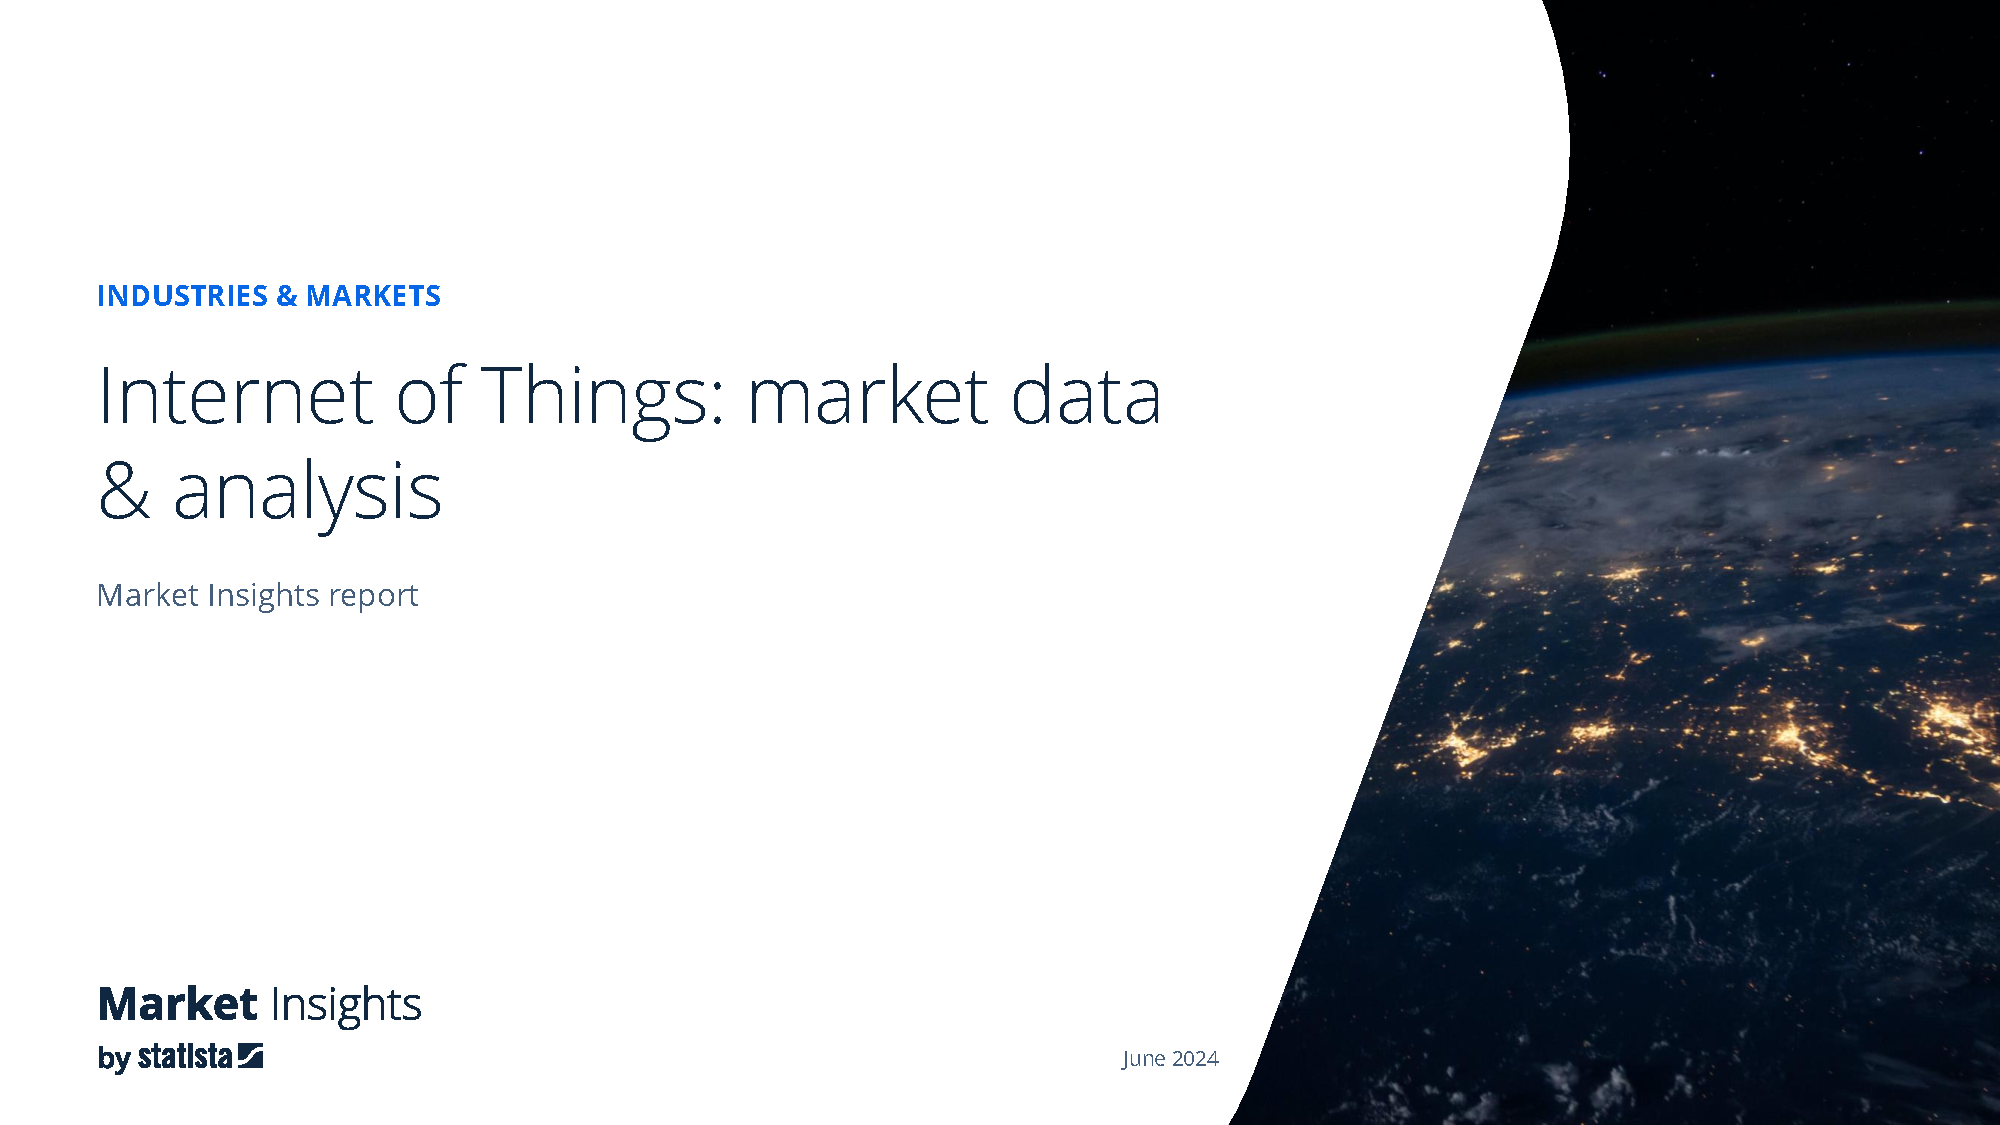
\includegraphics[width=0.9\textwidth]{Statista_iot.png}
	\label{IoT-Verbindungen}
\end{figure}



	\chapter{Netzwerkverbindungen von \ac{iot}-Geräten}
Zwei der am meistgenutzten Verbindungen zwischen \ac{iot}-Geräten sind Mesh-Netzwerke und Zigbee, die hier kurz beschrieben werden solle.
    
		\section{Mash-Netzwerk}
Der \ac{ieee} 802.11-Standard, welcher für \enquote{Standard für Informationstechnologie - Telekommunikation und Informationsaustausch zwischen Systemen - Lokale und Metropolen-Netzwerke - Spezifische Anforderungen Teil 11: Wireless LAN \ac{mac} und Physical Layer Spezifikationen} steht, hat für die Verwendung von Mesh-Netzwerken eine eigene Bezeichnung: \ac{ieee} 802.11s. Hierbei kommt es zu den oben genannten Titel der Zusatz \enquote{Änderung 10: Mesh-Netzwerk}. Beim \ac{ieee} 802.11s wird ein neues Routing-Verfahren eingesetzt, welches auf der \ac{mac}-Schicht anstatt auf der Netzwerkschicht, wie beim \enquote*{traditionellen} \ac{ieee} 802.11, durchgeführt wird. Dabei behält der \ac{ieee} 802.11s-Standard die physischen Schichten wie bei dem „traditionellen“ Standard. Um ein effizientes Routing zu haben, müssen die Knoten genaue Kenntnisse über die drahtlosen Verbindungen haben, die sie mit ihren direkten Nachbarn verbinden. Dies führt zu nahtlosem Routing für Protokolle höherer Schichten. In einem \ac{ieee} 802.11s-Mesh-Netzwerk, auch als \ac{mbss} bezeichnet, gibt es verschiedene logische Komponenten, wie in Abbildung \ref{Mesh} dargestellt. Die wichtigsten sind die Mesh-Stationen, die an der Bildung des \ac{mbss} teilnehmen und in dem jeder Knoten die gleiche Komplexität hat und keine hierarchische Struktur vorliegt. Die Mesh Stationen nehmen außerdem an der Pfadauswahl und -weiterleitung teil, wodurch ein sehr einfaches selbstorganisiertes Netzwerk entsteht.

            \begin{figure}[H]
           	\centering
	           \caption{Architektur eines Mesh-Netzwerkes}
	           \includegraphics[width=0.9\textwidth]{MeshNetwork}
		\label{Mesh}
            \end{figure}    

            Im Falle der Integration mit anderen Netzwerktypen, wie dem \enquote*{traditionellen} \ac{ieee} 802.11 oder wenn der \ac{mbss} auf externe Netzwerke zugreifen muss, sind andere logische Komponenten erforderlich. Die Geräte, welche den Zugang zum Mesh-Netzwerk für \enquote*{traditionelle} \ac{ieee} 802.11-Stationen gewährleisten, werden als Mesh APs bezeichnet. Darüber hinaus werden zur Kommunikation zwischen dem Mesh Netzwerk und einem nicht-\ac{ieee} 802.11 \ac{lan}, wie beispielsweise einem kabelgebundenen \ac{lan}, weitere logische Komponenten verwendet, nämlich die Mesh Portal Points, die die Kommunikation mit externen Entitäten ermöglichen \parencite[4-6]{Cilfone.2019}.  %Quelle Wireless Mesh Networking: An IoT-Oriented Perspective Survey on Relevant Technologies
            
		\section{Zigbee}
            ZigBee ist ein drahtloses Netzwerkprotokoll, das für niedrige Datenraten und niedrigen Stromverbrauch optimiert ist und hauptsächlich für die Automatisierung von Hausgeräten und anderen Geräten im \ac{iot} verwendet wird. Es wurde von der ZigBee Alliance entwickelt und basiert auf dem \ac{ieee} 802.15.4-Standard für \ac{pan}.
            Eines der wichtigsten Merkmale von ZigBee ist seine Fähigkeit, eine große Anzahl von Geräten mit geringem Stromverbrauch zu verbinden. Es ist auch sehr skalierbar und kann Netzwerke mit Hunderten von Geräten unterstützen. Die Sicherheit ist in ZigBee gut implementiert und es bietet auch eine hohe Zuverlässigkeit und geringe Latenzzeiten.
            ZigBee wird hauptsächlich in Anwendungen verwendet, in denen niedrige Datenraten und geringer Stromverbrauch erforderlich sind, wie beispielsweise in der Steuerung von Beleuchtung, Heizung und Klimatisierung, in Sicherheitssystemen und in der Überwachung von Umweltbedingungen. Es wird auch in vielen anderen Anwendungen im Bereich des Internet der Dinge verwendet, wie beispielsweise in der Industrieautomatisierung und in Gesundheitsüberwachungssystemen \parencite[195]{Gessler.2015}. %quelle Wireless-Netzwerke für den Nahbereich: Eingebettete Funksysteme: Vergleich von standardisierten und proprietären Verfahren

	
	\chapter{Angriffsszenarien}
 %Allgemeines zum Thema Angriffsszenarien
               
		\section{Ausnutzung von Fehlern in der Sicherheit von \ac{iot}-Geräten}
 Kein System ist von Grund auf perfekt. Mit der Zeit werden Systeme entsprechend geupdated und Sicherheitslücken werden geschlossen. Smart Home Geräte wie Kühlschränke, Glühbirnen oder ähnliches werden jedoch häufig von sicherheitsunkundigen Personen genutzt, nach dem Kauf an Strom und Internet angeschlossen und danach nicht weiter beachtet. Dadurch bleiben Sicherheitslücken bestehen, die sich schon bei der Produktion in den Geräten befunden haben. Solche Sicherheitslücken können dann von Hackern ausgenutzt werden. In den gleichen Bereich fallen auch standardmäßig gesetzte Passwörter, die in Handbüchern stehen, bei allen Geräten gleich sind und nicht geändert werden. Die Ransomwares WannaCry und NotPetya verursachten im Jahre 2017 Milliarden an Schäden, indem sie eine Schwachstelle in der Implementierung des Server Message Block Protokols von Microsoft ausnutzten \parencite[5]{Chantzis.2021}. Zum Zeitpunkt des Angriffs war der Fehler bereits bekannt und es stand seit 2 Monaten ein Hotfix von Microsoft zur Verfügung.
 
		\section{Spoofing}
  Beim Spoofing agieren Angreifer, als wären sie Teil des Netzwerkes oder als wären sie jemand anderes. Dies ermöglicht dem Angreifer sich zwischen zwei kommunizierende Geräte zu platzieren, die Übertragungen beider Seiten abzufangen und diese durch seine eigenen Übertragungen zu ersetzen. Diese Form wird Man-In-The-Middle-Angriff genannt.
Alternativ kann der Angreifer sehr viele Anfragen an einen Netzwerkteilnehmer schicken, wobei er die Daten des anfragenden Geräts fälscht. Die Antworten werden dann an diese gefälschte Adresse geschickt, mit dem Ziel diese Adresse mit den Antworten zu überlasten. Hier spricht man von einer Denial-of-Service-Attacke, oder wenn mehrere Geräte genutzt werden, um ein Ziel zu mit Antworten zu überfrachten, von einer Distributed-Denial-of-Service-Attacke.
  
		\section{Seitenkanalattacke}
  Nach Abrishami handelt es sich bei Seitenkanalattacken um nicht invasive Angriffe, da die Geräte dabei nicht zerstört oder verändert werden. Durch Beobachtung, Messungen, Abfangen von Funkdaten mit oder ohne Senden von Daten an das Gerät lassen sich Rückschlüsse auf interne Komponenten oder Berechnung durchführen. Unterschieden werden dabei sieben verschiedene Möglichkeiten der Seitenkanalattacke \parencite{Abrishamchi.2017}.
  
  Eine davon ist die Netzwerkverkehranalyse. Dabei werden die Pakete, die in einem Netzwerk von Geräten verschickt und empfangen werden, analysiert. Sender- und Empfänger\hyphen MAC\hyphen Adresse sind in jedem Paket nach \ac{ieee} 802.3 Standard im Klartext vorhanden und auslesbar. Dadurch lässt sich ermitteln welche Geräte untereinander kommunizieren. Durch die Größe der Pakete, Anzahl oder Zeitpunkte lassen sich weitere Details ermitteln.
  
  Zum Beispiel sendet ein Gerät, das auf Sprachbefehle wartet, regelmäßig Daten an einen Server, um die aufgenommenen Geräusche zu analysieren. Bei erhöhter Kommunikation des Geräts und Antworten des Servers liegt daher der Verdacht nah, dass gesprochen wird und sich mindestens eine Person im Raum befindet. Khan et. al. waren 2009 bei verschlüsselter Kommunikation in der Lage aus 10 Personen mit 70-75\% Wahrscheinlichkeit die sprechende Person zu identifizieren \parencite[70]{Khan.2010}.
		
	\chapter{Gründe für Angriffe auf \ac{iot}-Geräte}
 Gründe für das Angreifen von Teilen des \ac{iot} sind unterschiedlich und abhängig ob die Ziele bewusst ausgewählt werden, z.B. im Rahmen von Firmenspiongage, oder es sich um zufällige Ziele handelt, um ein Botnetzwerk aufzubauen.
 
		\section{Botnetze}
  Kleinere Gegenstände aus dem \ac{iot} haben bauartbedingt nicht die gleiche Rechenkapazität wie ein Desktop-PC oder ein Laptop/Tablet. Dies wäre auch völlig überdimensioniert. Da die Programme auf solchen Geräten gleichzeitig recht einfach sind und wenig Leistung erfordern ist jedoch freie Rechenkapazität vorhanden. Durch das Einbinden von solchen Kleinstrechnern in das Botnet kann über die reine Anzahl solcher Geräte ein profitables Botnetz entstehen. Im Bericht des \ac{bsi} aus dem Jahre 2015 steht, dass im Durchschnitt pro Tag 60.000 neue Systeme pro Tag allein in Deutschland infiziert werden. Nicht alle werden in Botnetze eingebunden oder bleiben übernommen, aber es besteht Potential \parencite[30]{BundesamtfurSicherheitinderInformationstechnik.20210106}. Mit der steigenden Anzahl an \ac{iot}-Geräten seit 2015 ist auch damit zu rechnen, dass sich diese Zahl vergrößert hat. Laut Putman haben Botnetze die Möglichkeit sechsstellige Summen oder noch höhere Beträge zu erwirtschaften \parencite{Putman.2018}. 
  
		\section{Einfallstore in Netzwerke}
  Beim Angriff auf Systeme gehen Hacker meist sehr gezielt und methodisch vor. Entsprechend greifen sie nicht zuerst die am stärksten gesicherten Teile eines Netzwerkes am, um in ein System einzudringen. Sondern sie versuchen sich zuerst an den weniger gesicherten Geräten, um Zugriff zu erlangen. Sobald ein Hacker Zugang zu einem schwächer gesicherten Gerät oder einer schwächer gesicherten Komponente erhalten hat, kann er sich von dort aus weiter ausbreiten und das System schrittweise infiltrieren. Entweder indem Informationen abgegriffen werden können, die die Attacke auf eine andere Komponente erlauben. Eine andere Möglichkeit besteht darin, das schwächere Gerät oder die schwächere Komponente als Basis zu verwenden, um die eigene Identität zu verschleiern und sich als eine andere Person oder ein anderes Gerät auszugeben. Hierbei kann der Hacker andere Teile des Systems manipulieren oder steuern, ohne erkannt zu werden.
  
		\section{Ausspähen von menschlicher Anwesenheit}
  Durch die Ausnutzung von Angriffen, die auf die Anwesenheit von Personen in Gebäuden hindeuten (siehe Seitenkanalattacken) können Objekte ausgekundschaftet werden, bzw. bestimmte Bereiche auf Anwesenheit überwacht werden.

\begin{figure}[ht]
	\centering
	\caption{Heatmap von Joggern in geheimer US Basis}
	\includegraphics[width=0.9\textwidth]{Heatmap.png}
	\label{Heatmap}
\end{figure} 
  
  Eine weitere Möglichkeit der Nutzung von solchen Erkenntnissen ist die Erstellung von Bewegungsprofilen von Personen. Hier sticht insbesondere die Verfolgung sogenannter Wearables (Smartwatches, Fitnesstracker o.ä.) hervor. Meist sind diese mit einem Mobiltelefon verbunden, tauschen regelmäßig Daten aus oder laden sie auf Webseiten hoch. Auf diese Weise wurde im November des Jahres 2017 eine geheime Afghanistan-Basis der US Armee enttarnt, als vom dem sozialem Fitnessnetzwerk Strava eine Heatmap mit 3 Billionen GPS-Punkten veröffentlicht wurde. Ein extrem heller Spot in einem ansonsten dunklem Gebiet in der Helmand Provinz in Afghanistan ließ dabei auf Anwesenheit schließen und die Heatmap war detailliert genug, um sogar das Layout der Basis in Erfahrung zu bringen. Kartendienste wie Google Maps zeigten an der gleichen Stelle keinerlei Aktivitäten \parencite{.20180128}. 

        
		\section{Spurenloser Einbruch}
        Zugangssysteme mittels \ac{rfid}-Tags, -Karten oder dem Mobiltelefon,  sowie biometrische Systeme haben auch in Privathaushalten Einzug erhalten und ersetzen den klassischen Schlüssel an der Haustür. Sind diese Systeme mit einer Basisstation verbunden, ist diese im Normalfall an das Internet angebunden und kann über bereits erwähnte Wege angegriffen werden, um so Zutritt zu erlangen. Es besteht aber auch die Möglichkeit mittels \ac{rfid}-Lesern den Inhalt des Zugangstokens auszulesen. Dazu genügt es oft schon den Leser für 1 bis 2 Sekunden in der Nähe des \ac{rfid}-Tags zu bringen. Anschließend können mittels verschiedener Programme oder eines Brute-Force-Angriffs den Inhalt der Sector Keys \footnote{Sector Keys sind Verschlüsselungsdaten, die den Zugriff auf bestimmte Sektoren des \ac{rfid}-Chips erlauben} ausgelesen werden und so eine funktionierende Kopie des Zugangstokens repliziert werden. Mit diesem kann dann die Tür normal geöffnet werden, ohne das Einbruchsspuren zurück bleiben. Eventuell vorhandene Alarmsysteme können zudem häufig mit einem Störsender überlagert werden, indem ein weißes Rauschen auf den verwendeten Frequenzen gesendet wird.

Ein entsprechender Angriff inklusive verwendeter Soft- und Hardware wird in \citetitle{Chantzis.2021} auf den Seiten 372-379 ausführlich dargelegt.

	\chapter{Fazit}
Die vorliegende Arbeit hat sich mit den technischen Vorraussetzungen von IoT-Geräten in behördlichen Infrastrukturen beschäftigt. Dabei wurde deutlich, dass mit der zunehmenden Verbreitung von IoT-Technologien neue sicherheitsrelevante Herausforderungen entstehen, denen Rechnung getragen werden muss.

Ein zentrales Ergebnis der Analyse ist, dass insbesondere schlecht gesicherte oder veraltete IoT-Geräte als Einfallstor für Angriffe dienen können. Angriffsszenarien wie Spoofing, Seitenkanalattacken oder das Auslesen von RFID-Tags zeigen, dass der Zugriff auf sensible Bereiche teilweise mit einfachsten Mitteln möglich ist – oft ohne Spuren zu hinterlassen. Auch die Nutzung kompromittierter Geräte in Botnetzen stellt ein erhebliches Risiko dar. Die beschriebenen technischen Grundlagen zeigen wie die Kommunikationsstrukturen der \ac{iot}-Geräte beschaffen sind.

Die Ergebnisse unterstreichen die Notwendigkeit, Sensibilisierung und Schulung von Mitarbeitenden in Bezug auf IoT-Sicherheit auszubauen sowie konkrete technische Maßnahmen – wie das Monitoring von Funkverbindungen und das konsequente Patchen von Geräten – umzusetzen. Für Behörden wie das \ac{rzf} könnte dies bedeuten, dass zukünftig eigene Richtlinien und Frühwarnsysteme für IoT-Risiken etabliert werden müssen.

\newpage %Abschluss Inhalt - Neue Seite für Anhänge
%\nocite{*}
\printbibliography[heading=bibintoc, title={Literaturverzeichnis}] %Erzeuge Literaturverzeichnis
%\appendix %Anhänge
\end{document}
